

%%%%%%%%%%%%%%%%%%%%%%%%%%%%%%%%%%%%%%
%
% This is how you write code:
%
% \begin{minted}{matlab}
% foo = [2 1 0;1 4 3;2 4.5 6];
% \end{minted}
%

% This is how you import code:
% 
% \inputminted[linenos]{matlab}{foo_bar.m}
%
 
% Most figures are imported this way:
%
% \begin{figure}
% \includegraphics[width=\textwidth]{foo_figure}
% \caption{This is a caption}
% \end{figure}
%
%%%%%%%%%%%%%%%%%%%%%%%%%%%%%%%%%%%%%%


\documentclass[00-main.tex]{subfiles}
\begin{document}


\subsection*{1b)}

In the following, \textsc{Matlab} is used to solve \cref{eq: Grad(W)} with both the forward (\cref{forw}) and backward (\cref{back}) Euler method.

\begin{equation}
\label{forw}
\tilde{W}_{k+1}=W_k - \alpha(G_k-W_k G_{k}^{T}W_k), \quad G_k:=\frac{\partial \phi}{\partial W}_{W=W_{k}}
\end{equation}
\begin{equation}
\label{back}
\tilde{W}_{k+1}=W_k - \alpha(G_{k+1}-W_{k+1} G_{k+1}^{T}W_{k+1}),\quad G_{k+1}:=\frac{\partial \phi}{\partial W}_{W=W_{k+1}}
\end{equation}

Here the step size is $\alpha$ - and each step in the implicit backward Euler method is solved by applying fixed point iteration.

Comparing the two methods to the differential equation system above, one can see that the methods assume orthogonality in that $W_{k}^{T}W_k=I$. Each step doesn't necessarily produce a resulting orthogonal matrix $\tilde{W}_{k}^{T}\tilde{W}_k=I$. Therefore, our implementation of the method allows one to perform the projection that 
\begin{equation}
W_{k+1}=Q, \quad \text{where} \quad \tilde{W}_{k+1}=QR
\end{equation}

by QR decomposition.

The principle behind solving the system in \cref{eq: Grad(W)} is that the sum of independent variables has a distribution closer to the Gaussian distribution, according to the central limiting theorem. The system can be used to approximate the maximum non-aussianity, as the assumption is that when the system is furthest from Guassianity it will sort out the original components. For simplicity our methods require a mean of 0, and the assumption is that the signals are statistically independent with unit variance. The estimated sources will abide by this assumption and return solutions with mean=0 and variance=1.
Consider the three signals shown in \cref{source}. 
These signals represents speaker signals that have been transformed to a mean of 0 with unit variance. 
By having a minimum of three microphones that record superpositions of the signals, one can use the solution of the problem posed in \cref{eq: Grad(W)} to find a demixing matrix used to estimate the original sources from the signals each microphone record.

\begin{figure}[!htbp]
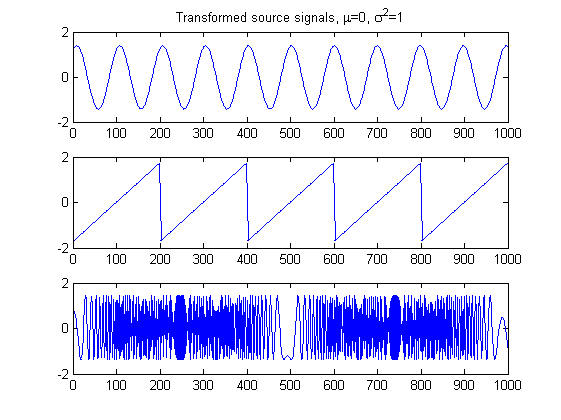
\includegraphics[scale=0.83]{transformedsourcesignals.png}
\caption{Plot showing the three source signals}
\label{source}

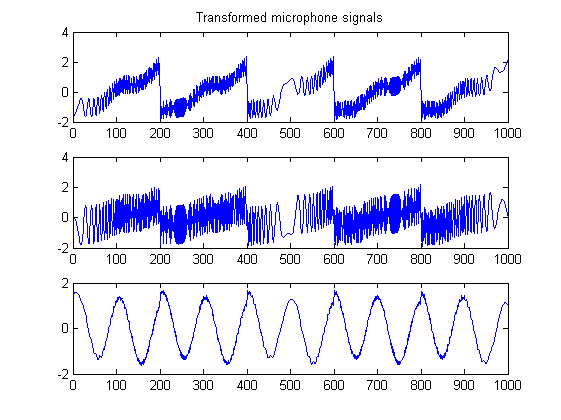
\includegraphics[scale=0.83]{transformedmicsignals.png}
\caption{Plot showing the transformed signals after mixing}
\label{mic}
\end{figure}

The superpositioned signals that each microphone records are plotted in \cref{mic}. Note that in the plot, the signals have been transformed using a whitening procedure such that $E[\tilde{x}\tilde{x}^T]=I$. 

This way $W$, found through the Euler methods, will be an orthogonal de-mixing matrix (given that QR-projection is applied, otherwise it will not be orthogonal) that can be used to find estimates $y$ of the original sources:

\begin{equation}
\label{y}
y(t) := W^T\tilde{x}(t)
\end{equation}

The estimated source signals after demixing are plotted in the following figures depicting the forward (\cref{forward}) and backward (\cref{back}) Euler method. 


\begin{figure}[!htbp]
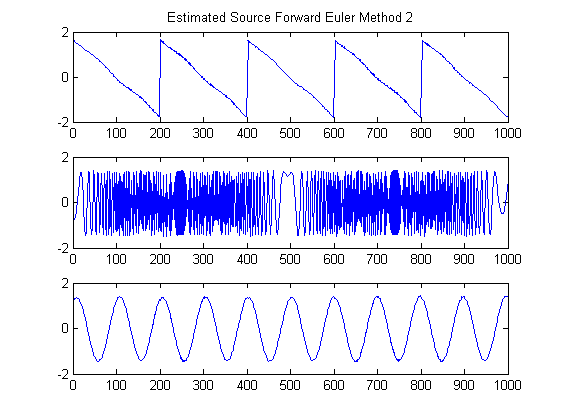
\includegraphics[scale=0.86]{estsignalsforward.png}
\caption{Plot showing the estimates of the original sources by the forward Euler method}
\label{forward}

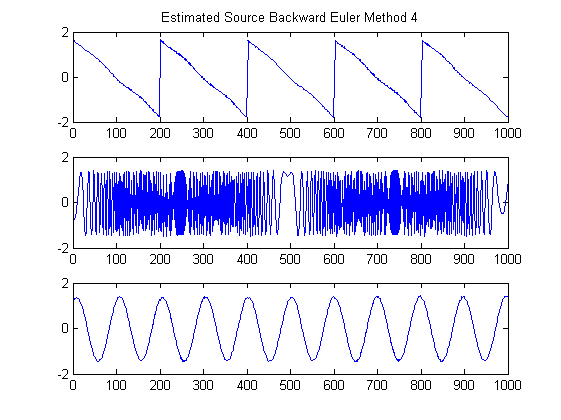
\includegraphics[scale=0.86]{estsignalsbackward.png}
\caption{Plot showing the estimates of the original sources by backward Euler method}
\label{back}
\end{figure}

The plots look reasonably similar to the original sources. One can note that the signals weren't necessarily returned in the order they were put in, nor were they always returned with the correct sign, meaning solutions may appear with their phase inverted. We noted similar effects for several other mixing-matrices.

When applying the forward Euler method without the QR-projection for orthogonality in each step, the result didn't converge towards any reasonable demixing matrix. This is not surprising, since \cref{forw} assumes orthogonality from \cref{eq: Grad(W)}.

The variables in the implementation of the Euler method is the step-size $\alpha$ and whether to apply the forward or backward method. By testing different step-sizes we found that larger step-sizes requires less iterations of the Euler methods, naturally. And as long as the step-size is reasonably small (for the speaker signals $\alpha$ should be less than $0.5$), $W$ converged nicely. The backward Euler-method implementation includes a fixed-point iteration loop for each step of the method, which gives it an extra dimension of iterations. We didn't encounter any stability issues with the forward Euler method, therefore the extra iterations of the backward Euler method made it a comparatively slower method for finding the demixing matrix W. 

One can use the error measure
\begin{equation}
E_k := |\phi(W_k) - \phi(W_{k-1})|
\end{equation}

to observe the rate at which $\phi(W_k)$ approaches a minimum. The plots below (\crefrange{01}{0005}) show $E_k$ plotted for step-sizes 0.1, 0.02 and 0.005. As one can see from the plots, the difference from each $\phi(W_k)$ to the next starts out smaller for the smaller step sizes, but the larger step sizes quickly surpass the smaller ones to reach the smaller differences faster.

\begin{figure}[!htbp]
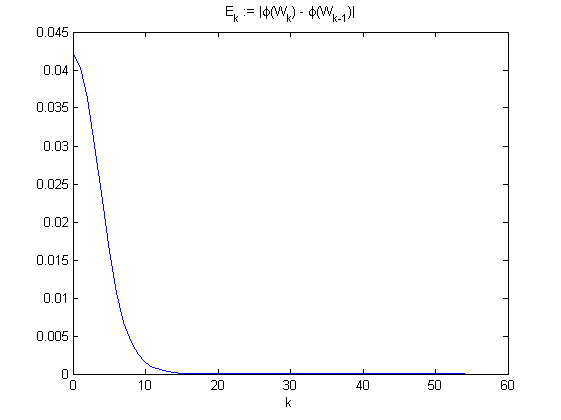
\includegraphics[scale=0.86]{errorstep01.png}
\caption{Plot showing the error for $\alpha=0.1$}
\label{01}

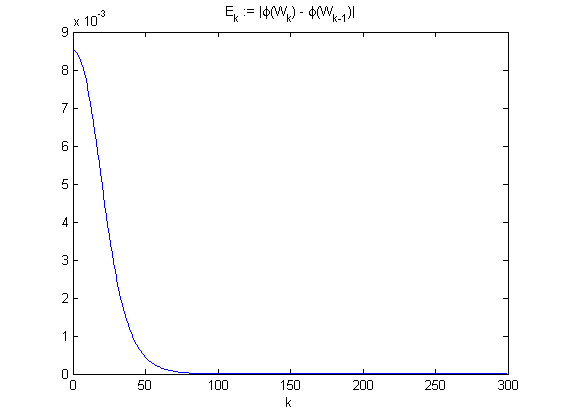
\includegraphics[scale=0.86]{error002.png}
\caption{Plot showing the error for $\alpha=0.02$}
\label{002}
\end{figure}

\begin{figure}
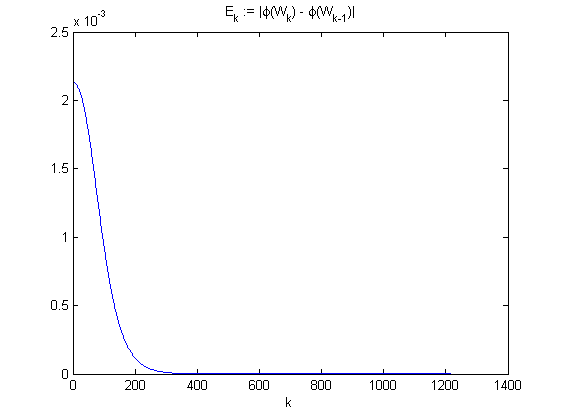
\includegraphics[scale=0.86]{error0005.png}
\caption{Plot showing the error for $\alpha=0.005$}
\label{0005}
\end{figure}


\clearpage
\subsection*{1c)}

The \textsc{Matlab} script imggen.m takes 3 grayscale pictures with positive kurtosis and turns them into \textsc{Matlab} vectors containing information about the degree of black/white in each pixel of the picture. These 3 pictures can then be mixed in the same way that the signals from 1b were mixed, and again demixed by solving the differential equation system with Eulers Method.
\cref{pappa} shows three grayscale pictures on the first line, the superposition mix on the second from a random mixing matrix, and the estimated signals after de-mixing on the last line. Just as the sign was not always correct on the speaker signals, wrong sign results in an inverted image, as one can see on the picture on the bottom, left. The images on the bottom row were produced with the forward Euler method using the \textsc{Matlab} function makeimg.m which takes the transformed signals from imggen.m as the argument.


\begin{figure}[!htbp]
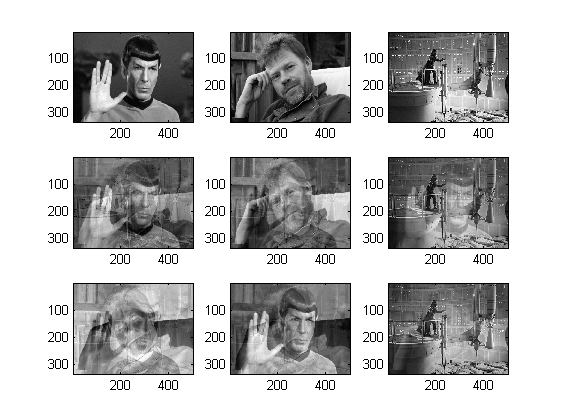
\includegraphics[scale=1]{pappa.png}
\caption{The pictures}
\label{pappa}
\end{figure}


The whole point of the differential equation system was to solve the optimization problem $\max_{(W \in O)} \phi(W)$. The definition of $\phi$ being
\begin{equation}
\phi(W)=\pm \frac{1}{4}\sum^{n}_{i=1}kurt(\mathbf(w)_{i}^{T}\tilde{x})
\end{equation}

Kurtosis is a measure of peakedness for a given distribution. Since we are trying to find solutions further from the Gaussian distribution, kurtosis can be used to decide how close our solution is to the Gaussian distribution, which is what $\phi(W)$ does. Depending on the sign in front of the sum, the problem becomes a maximum or minimum problem. \cref{phiW} shows the progression of $\phi(W_k)$ for the images, and because of $\phi$s connection with kurtosis, it illustrates the optimization of the kurtosis.


\begin{figure}
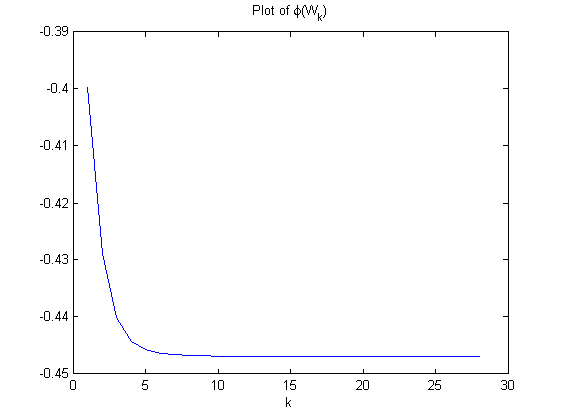
\includegraphics[scale=0.8]{phiW.png}
\caption{Progression of $\phi(W_k)$ }
\label{phiW}
\end{figure}

\end{document}

